{\begin{a3pages}
% ---------------------------------------------------------------------------- %
\section{\Master}
\label{sec:hw:master}
% ---------------------------------------------------------------------------- %
    % \parindent is set to 0 inside of minipages. Back up its value and access
    % it inside the minipage.
    \setlength{\parindentbak}{\parindent}

    \noindent\adjustbox{valign=t}{\begin{minipage}{135mm}
        Das \Master~ (Abbildung  \ref{fig:hw:master:photo:master}) basiert auf
        einem  \Raspi~ (Abbildung  \ref{fig:hw:master:photo:raspi}), erweitert
        mit einem zugekauften Touchscreen-Modul  und einem eigens entwickelten
        PCB, welches  f\"ur zus\"atzliche Funktionalit\"at  verantwortlich ist
        (Kommunikation mit Sensoren, Strommessung, GSM-Modem).

        \setlength{\parindent}{\parindentbak} % restore paragraph indentation

        Montiert    ist    das     \Master~in    einem    Hutschienengeh\"ause
        (auch       bekannt       als      DIN-Rail-Geh\"ause,       Abbildung
        \ref{fig:hw:master:photo:dinrail}). Damit   unser   Ger\"at   sinnvoll
        in    dem   Geh\"ause    untergebracht   werden    kann,   ist    eine
        eigene   Frontplatte  entwickelt   und  gefertigt   worden  (Abbildung
        \ref{fig:hw:master:photo:dinrailCover}).

        {\centering
            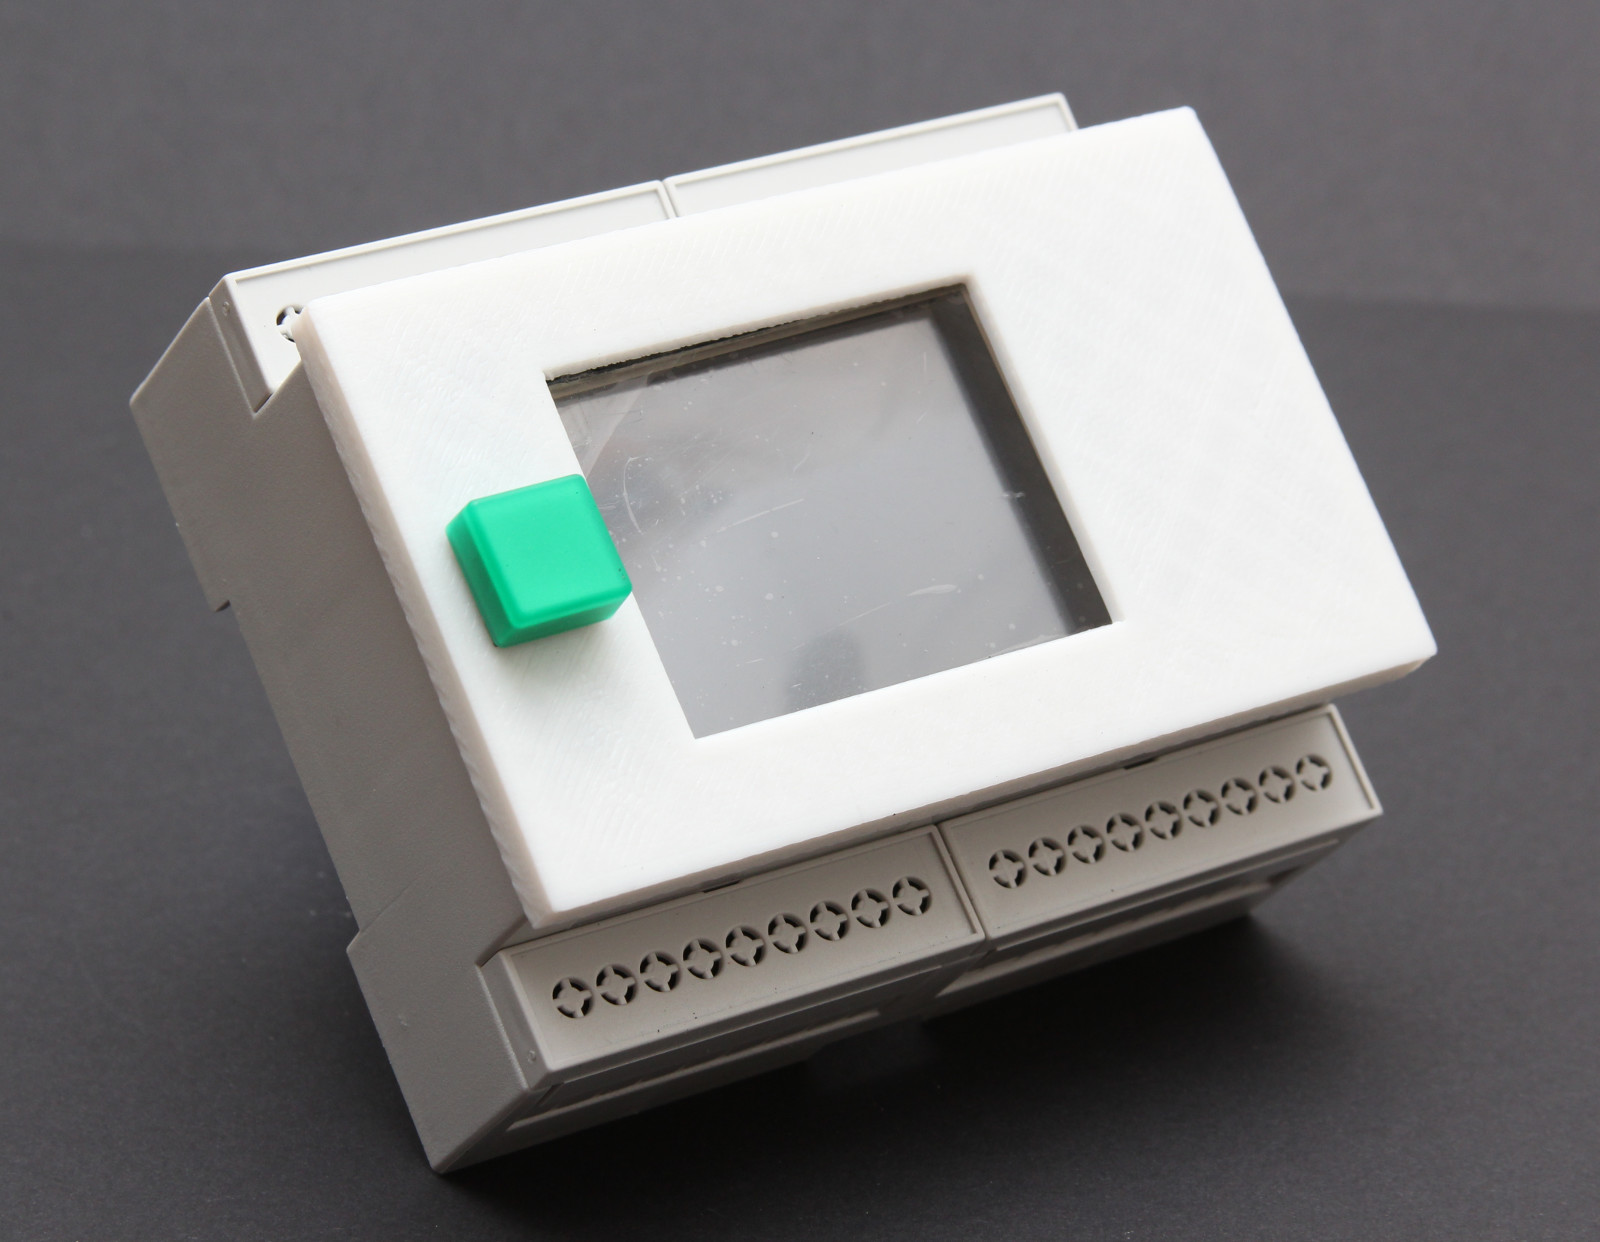
\includegraphics[width=100mm]{images/superv-photos/master.jpeg}
            \figcaption[\Master: Foto zusammengesetzt]{\Master, zusammengesetzt}
            \label{fig:hw:master:photo:master}
            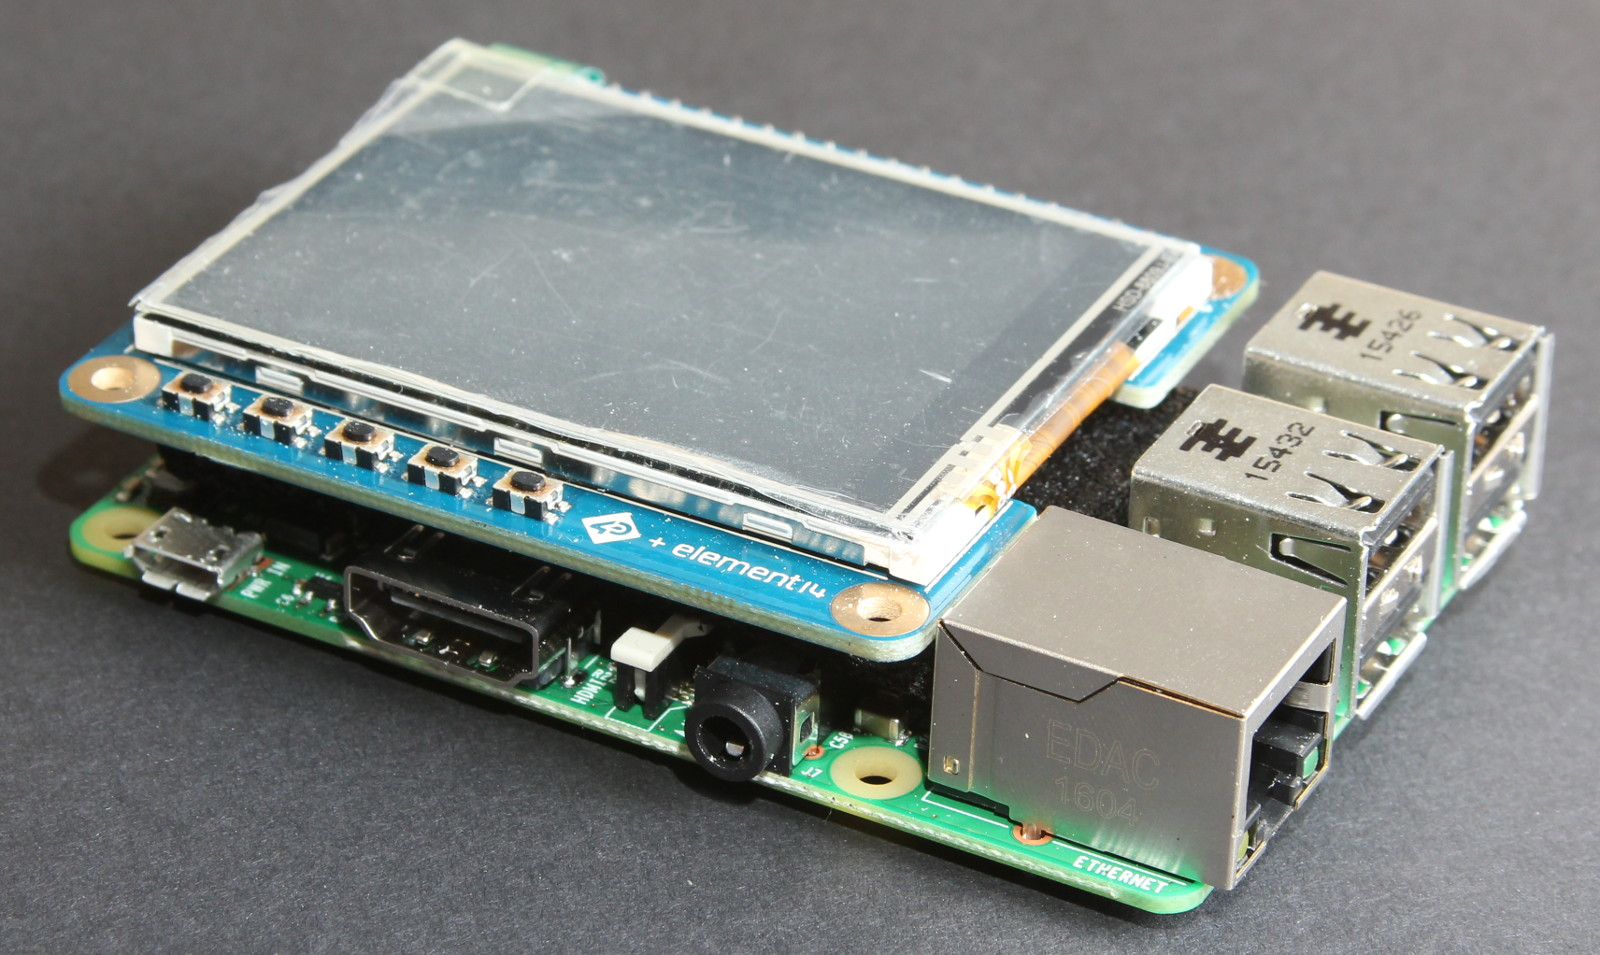
\includegraphics[width=100mm]{images/superv-photos/raspi-1.jpeg}
            \figcaption[\Master: Foto Touchscreen-Modul]{\Raspi mit aufgestecktem Touchscreen-Modul}
            \label{fig:hw:master:photo:raspi}
        }
    \end{minipage}}
    \hspace*{15mm}
    \adjustbox{valign=t}{\begin{minipage}{195mm}
        \centering
        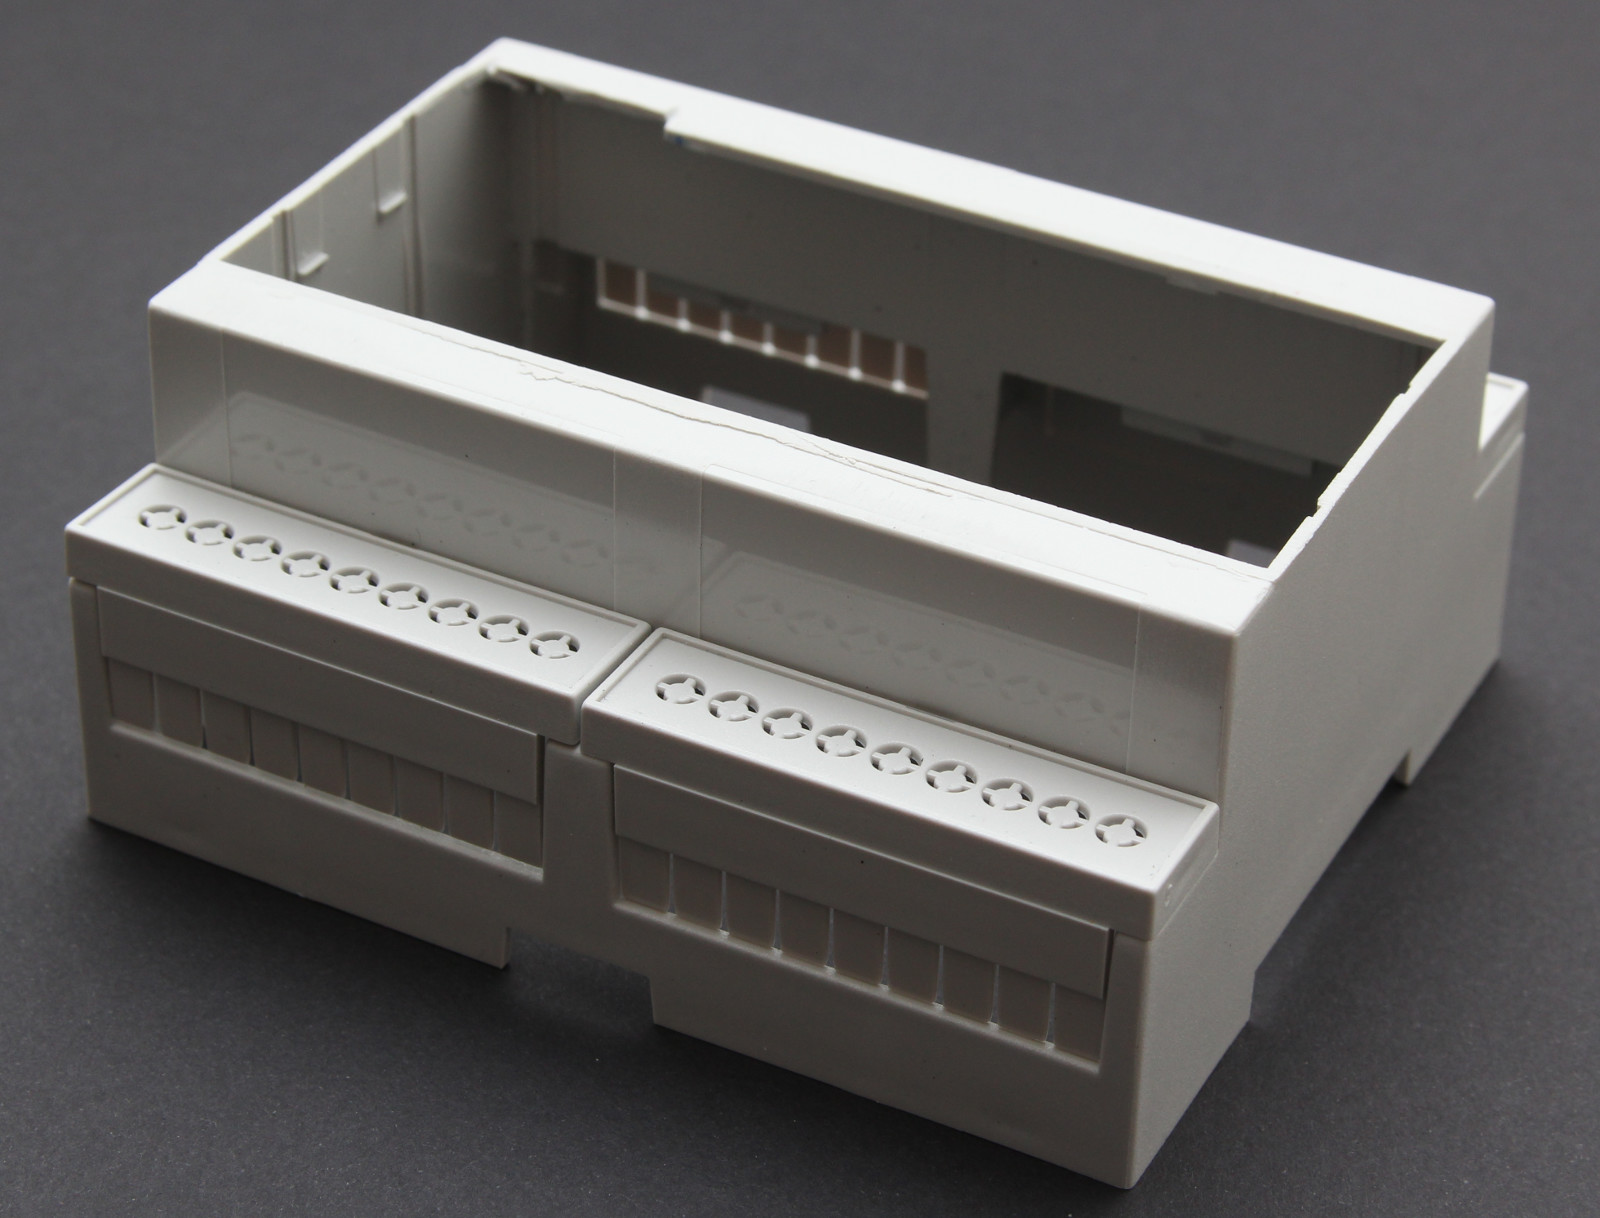
\includegraphics[width=100mm]{images/superv-photos/dinrail.jpeg}
        \figcaption[\Master: Foto Hutschienengeh\"ause]{Hutschienengeh\"ause}
        \label{fig:hw:master:photo:dinrail}
        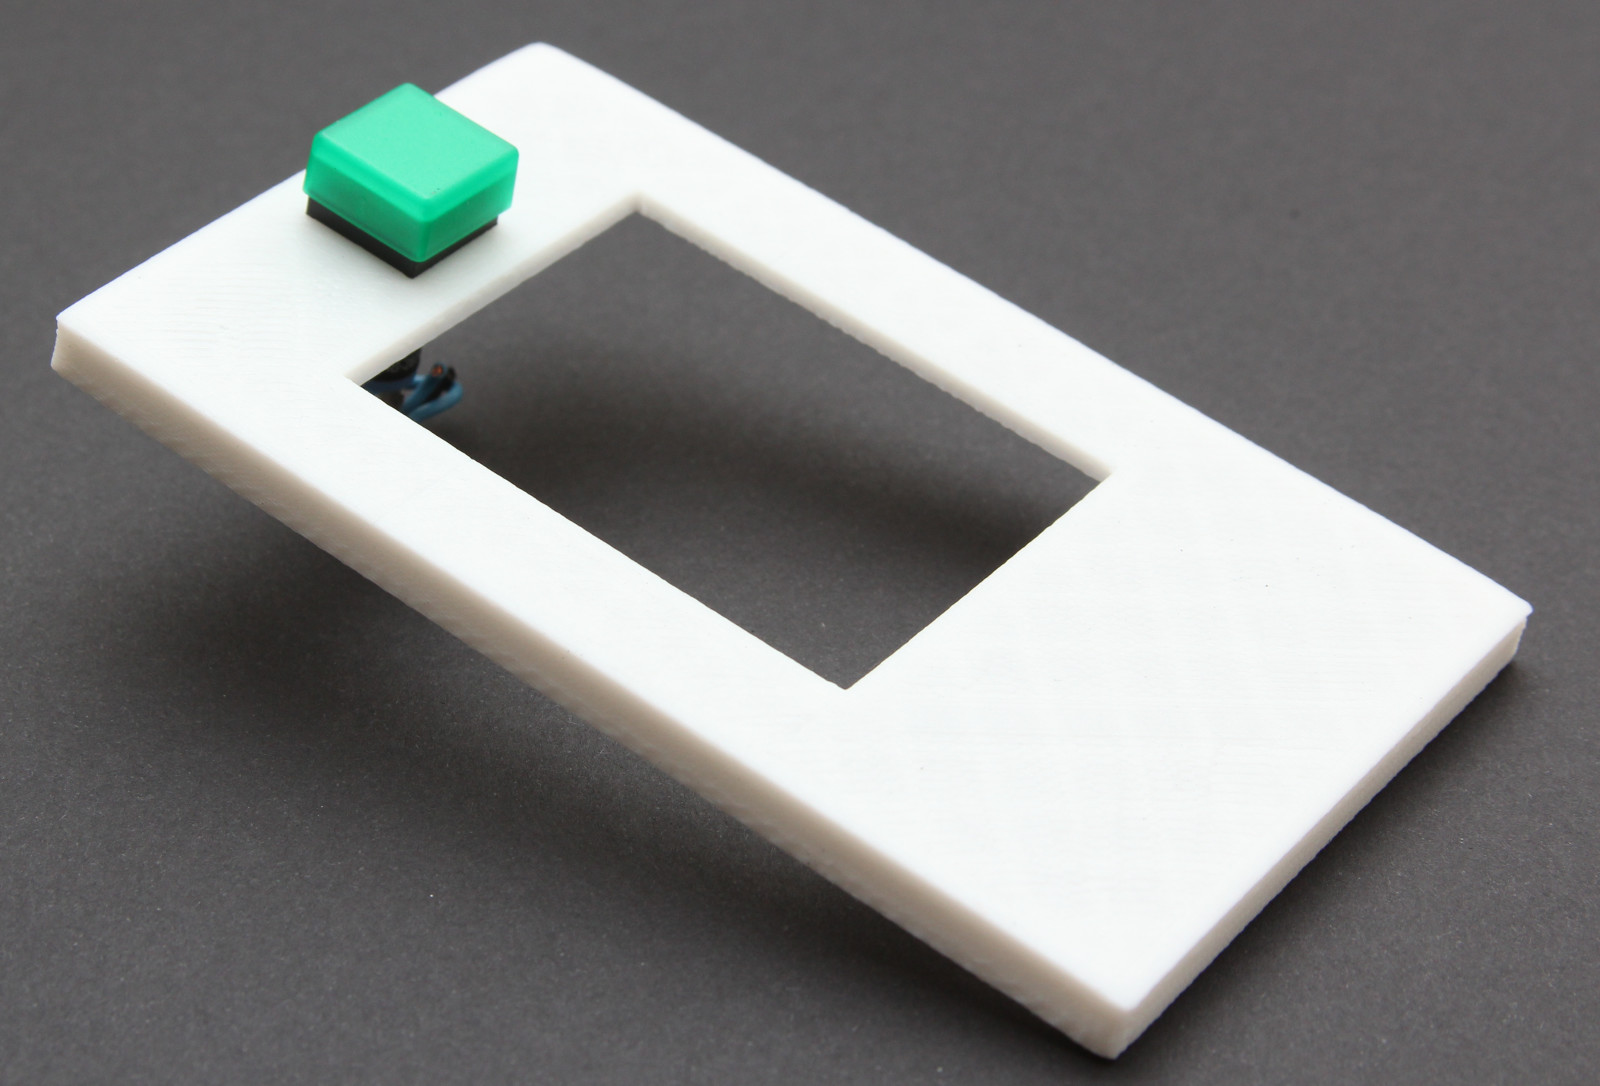
\includegraphics[width=100mm]{images/superv-photos/dinrail-cover.jpeg}
        \figcaption[\Master: Foto Abdeckung]{3D-degruckte Abdeckung f\"ur das Hutschienengeh\"ause}
        \label{fig:hw:master:photo:dinrailCover}
    \end{minipage}}

    \noindent\adjustbox{valign=t}{\begin{minipage}{135mm}
        Abbildung  \ref{fig:master:schema:highlights} zeigt  das Schema  f\"ur
        das   Zusatz-PCB   des  \Master   s. Bereich   1   ist  die   Speisung
        (genauer   dokumentiert  in   Abschnitt  \ref{subsec:hw:master:supply}
        ab  Seite  \pageref{subsec:hw:master:supply}),   allgemeine  Ein-  und
        Ausg\"ange   sind  im   Bereich  2   untergebracht  (siehe   Abschnitt
        \ref{subsec:hw:master:gpio} ab Seite \pageref{subsec:hw:master:gpio}),
        die  Kommunikation  mit den  Sensoren  erfolgt  durch die  Schaltungen
        in    Bereich     3    (Abschnitt    \ref{subsec:hw:master:sensorcomm}
        ab    Seite     \pageref{subsec:hw:master:sensorcomm})    der    Strom
        wird      mit       den      Komponenten      aus       Bereich      4
        gemessen    (Abschnitt    \ref{subsec:hw:master:current}   ab    Seite
        \pageref{subsec:hw:master:current})  und  Bereich   5  beinhaltet  die
        GSM-Schaltung    (Abschnitt   \ref{subsec:hw:master:gsm}    ab   Seite
        \pageref{subsec:hw:master:gsm}).

        \setlength{\parindent}{\parindentbak} % restore paragraph indentation
        Abbildungen  \ref{fig:master:pcb:front} und  \ref{fig:master:pcb:back}
        zeigen  ein  3D-Modell  des  PCB,  auf  welchem  die  Zusatzfunktionen
        untergebracht sind.

        Das  PCB  in  der  aktuellen Konfiguration  kann  drei  Modulstr\"ange
        parallel  verwalten. Das  Hinzuf\"ugen  zus\"atzlicher  Modulstr\"ange
        w\"are  relativ einfach,  w\"urde  aber ein  gr\"osseres  PCB mit  den
        zugeh\"origen zus\"atzlichen Komponenten bedingen.

        \adjustbox{valign=t}{\begin{minipage}{0.475\textwidth}
            \centering
            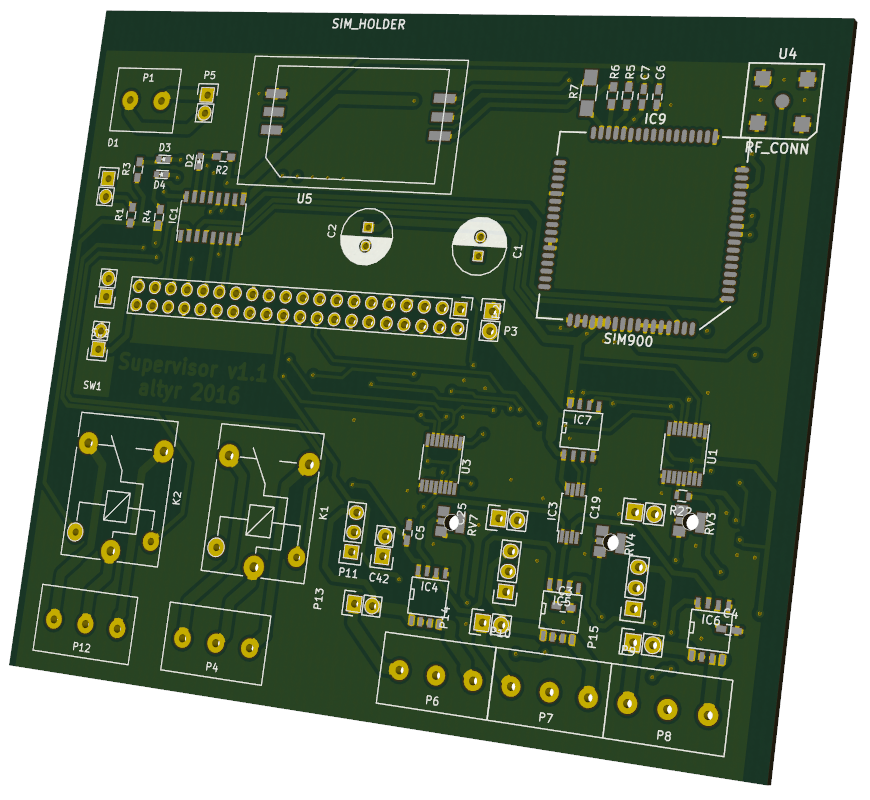
\includegraphics[width=0.9\textwidth]{images/superv-pcb/supervisor-3d-1.png}
            \figcaption[\Master: Vorderseite PCB]{PCB, Vorderseite}
            \label{fig:master:pcb:front}
        \end{minipage}}
        \adjustbox{valign=t}{\begin{minipage}{0.475\textwidth}
            \centering
            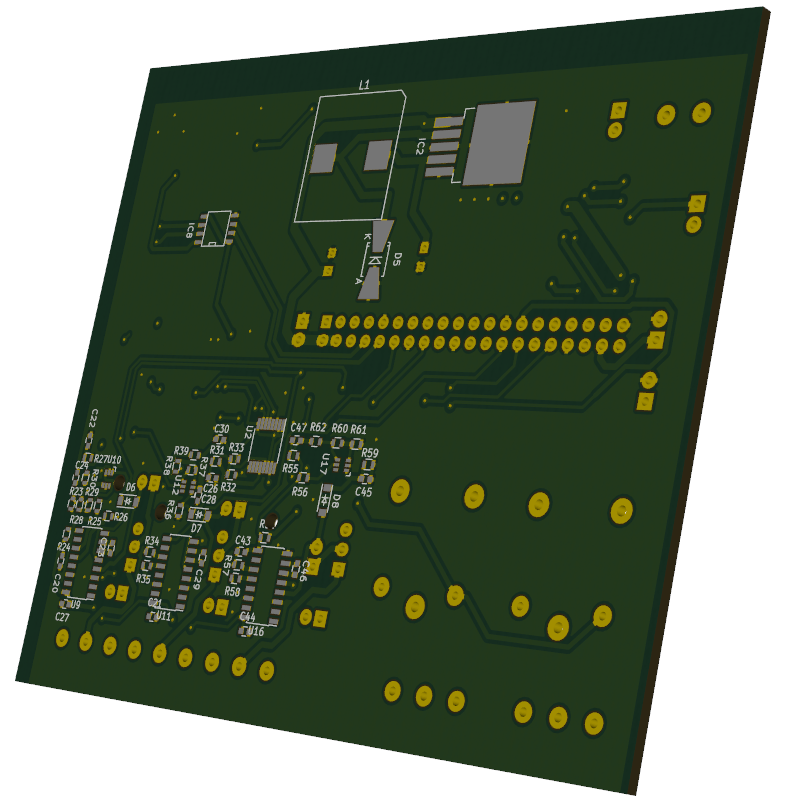
\includegraphics[width=0.9\textwidth]{images/superv-pcb/supervisor-3d-2.png}
            \figcaption[\Master: R\"uckseite PCB]{PCB, R\"uckseite}
            \label{fig:master:pcb:back}
        \end{minipage}}
    \end{minipage}}
    \hspace*{15mm}
    \adjustbox{valign=t}{\begin{minipage}{195mm}

        \centering
        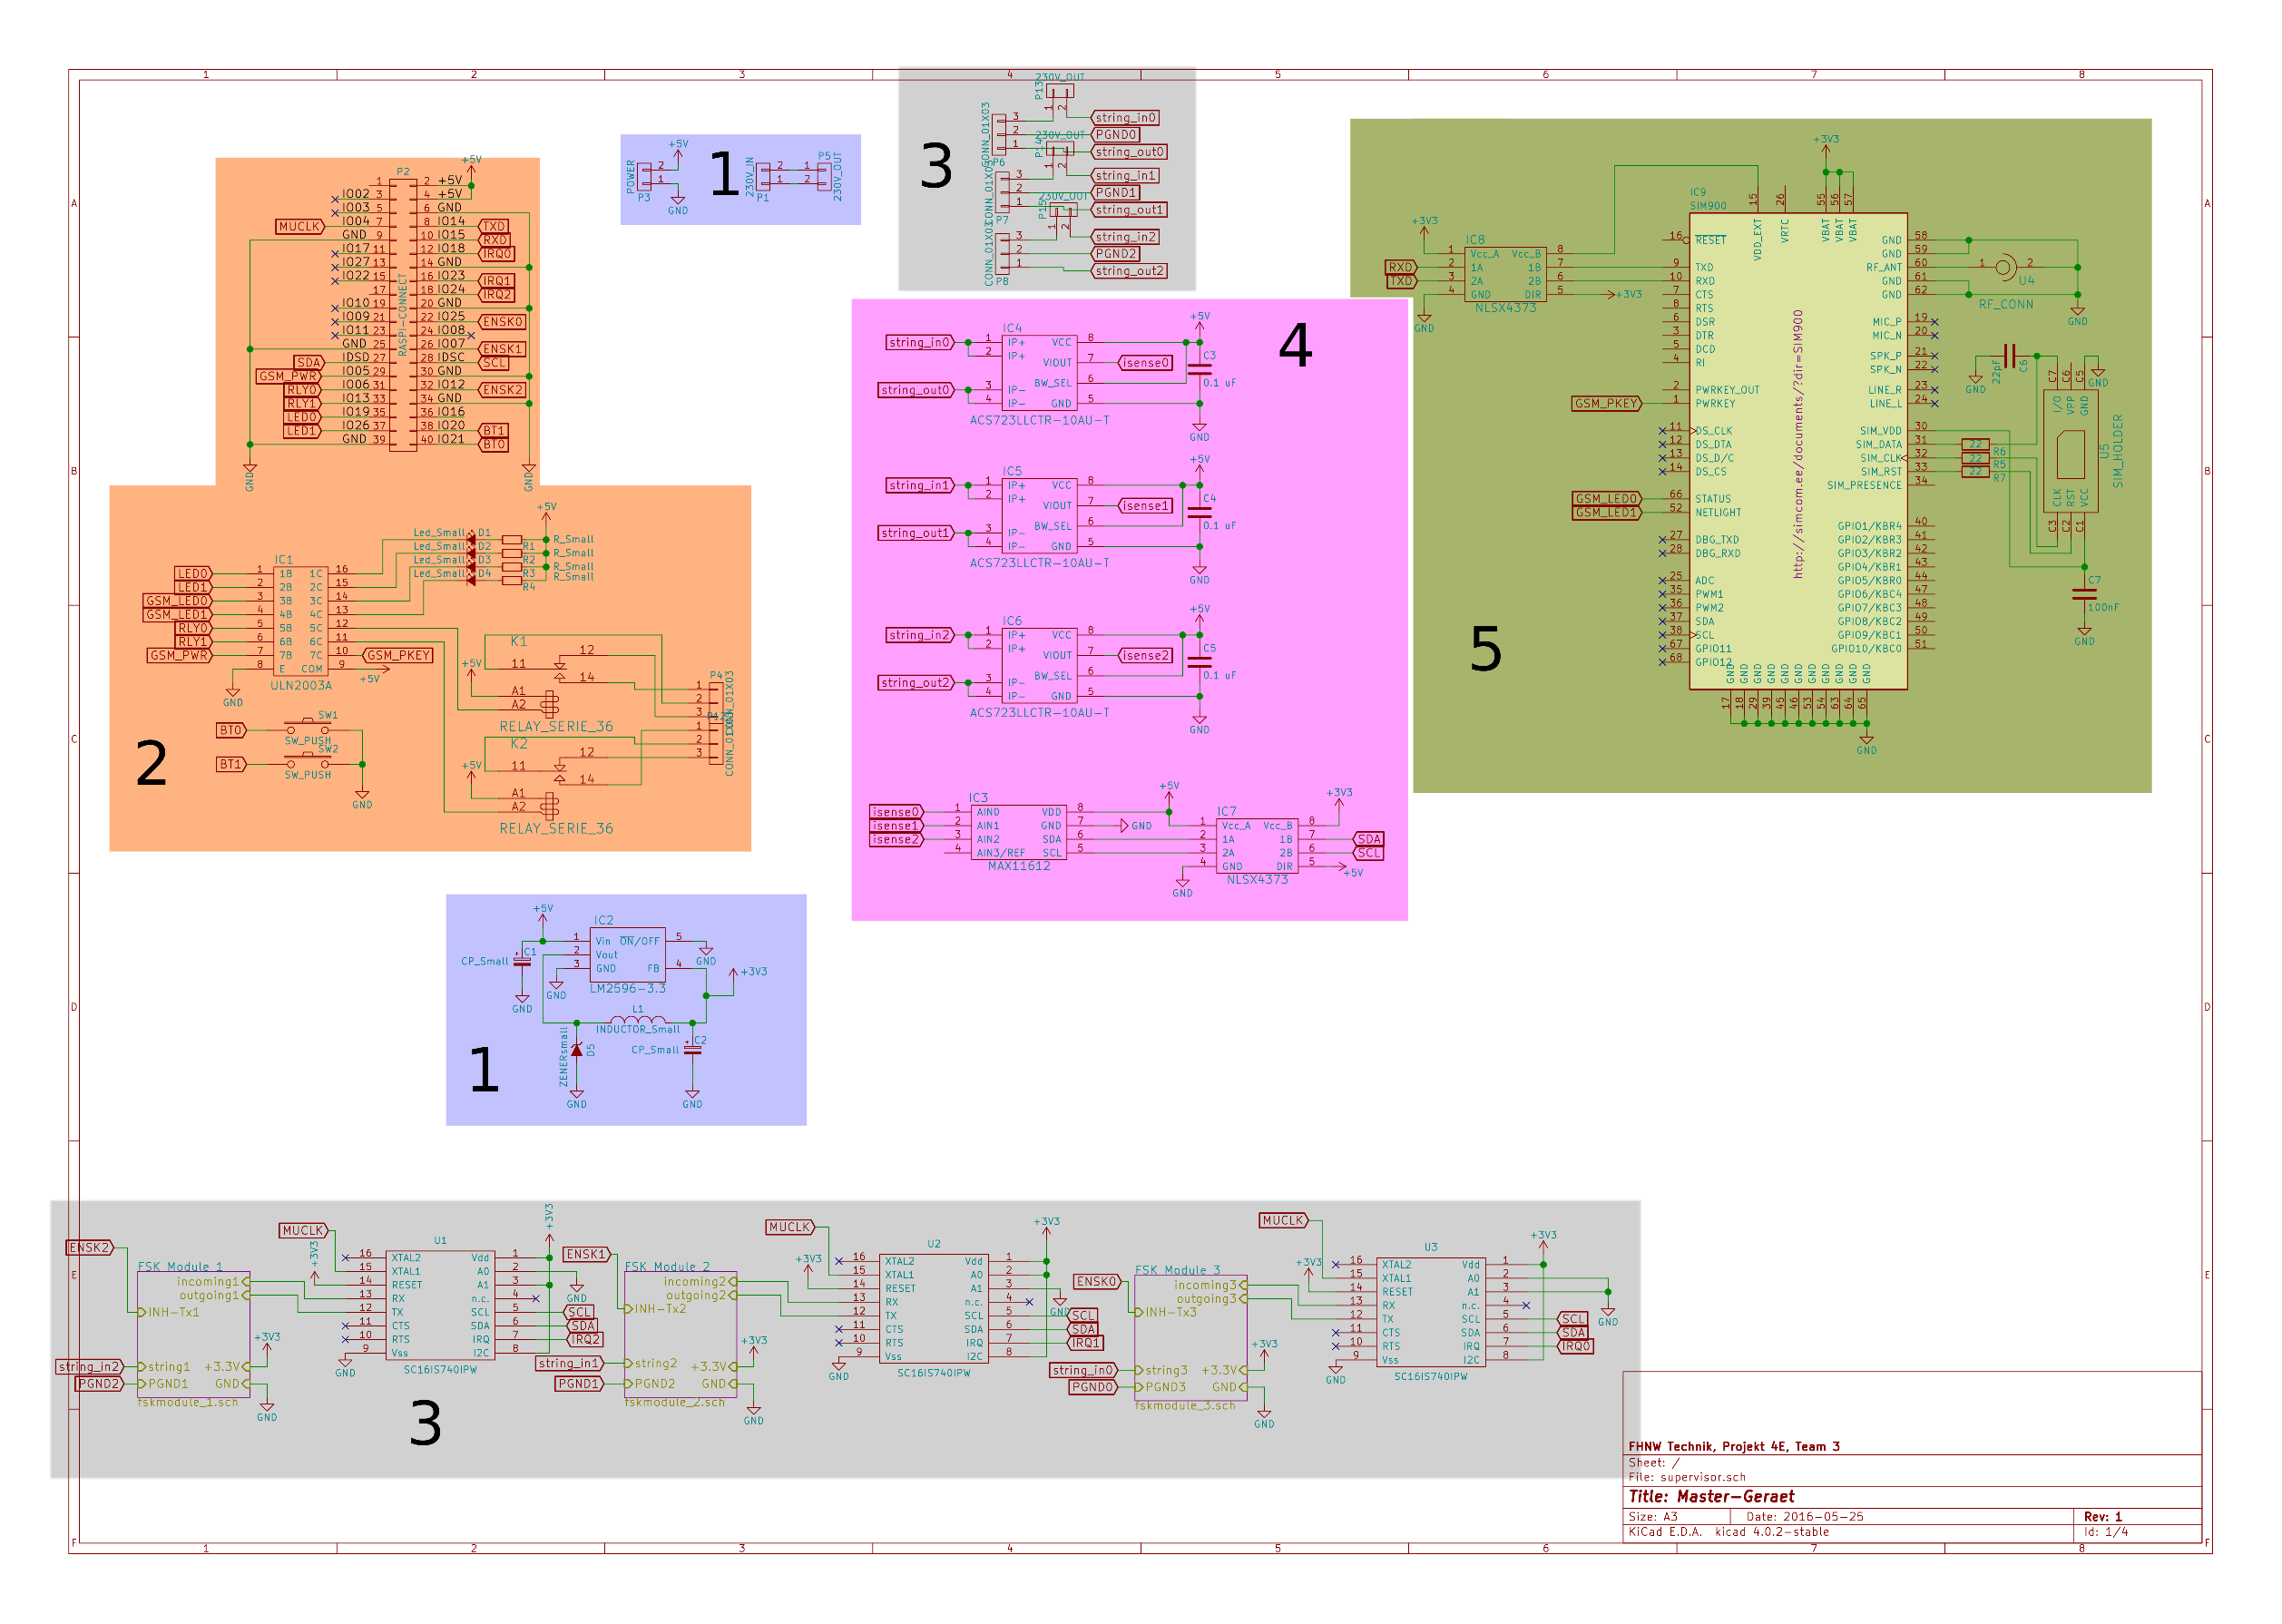
\includegraphics[width=\textwidth]{images/superv-sch/supervisor--sch--highlights.eps}%
        \figcaption[\Master: Schema, \"Ubersicht]{%
            Schema  des  Master-Ger\"ats. Eine   Grossversion  ist  in  Anhang
            \label{app:chap:schemas}  zu  finden,   die  einzelnen  Baugruppen
            sind  in  den  folgenden  Abschnitten  beschrieben  und  gr\"osser
            abgebildet.%
        }
        \label{fig:master:schema:highlights}

    \end{minipage}}
\end{a3pages}}


% ---------------------------------------------------------------------------- %
\subsection{Speisung}
\label{subsec:hw:master:supply}
% ---------------------------------------------------------------------------- %

\begin{figure}[h!t]
    \centering
    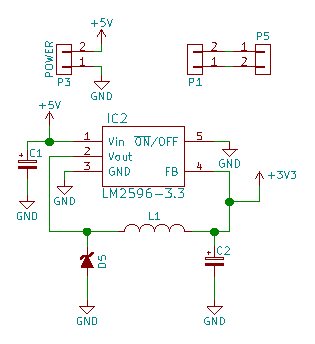
\includegraphics[width=0.33\textwidth]{images/superv-sch/supervisor--sch--supply.eps}
    \caption[\Master: Schema Stromversorgung]{Stromversorgung \Master}
    \label{fig:sch:master:supply}
\end{figure}

Die  Energie wird  vom  \SI{230}{\volt}-Netz bezogen  und  von einem  externen
Netzteil auf \SI{5}{\volt} transformiert. Aus  Platzgr\"unden und aufgrund der
Form des Geh\"auses wird der Netzanschluss dabei zuerst auf das PCB gef\"uhrt,
anschliessend  zum   Netzger\"at  weggef\"uhrt,  welches   dann  \SI{5}{\volt}
zur\"uckliefert.

F\"ur   Bauteile,  welche   \SI{3.3}{\volt}  Versorgungsspannung   ben\"otigen
(GSM-Modem,  \ldots),  ist  eine   Spannungswandlung  mit  einem  Schaltregler
implementiert   (\code{IC2}   und   zugeh\"orige  Komponenten   in   Abbildung
\ref{fig:sch:master:supply}). Der Schaltregler  ist das \SI{3.3}{\volt}-Modell
des LM2596 von \emph{Texas Instruments}.

Hauptverbraucher   auf   der   \SI{3.3}{\volt}-Schiene   ist   das   GSM-Modem
(siehe     Abschnitt     \ref{subsec:hw:master:gsm}),     welches     gem\"ass
Datenblatt~\cite{ref:sim900:1}~bis   zu    \SI{2}{\ampere}   bezieht. Es   ist
daher  wichtig,  dass   die  Spannungsversorgung  der  \SI{3.3}{\volt}-Schiene
gen\"ugend  Strom  liefern  kann. Der  ausgew\"ahlte  Regler  kann  bei  einer
Versorgungsspanunung   von  \SI{5}{\volt}   und  einer   Ausgangsspannung  von
\SI{3.3}{\volt} bis  zu \SI{3}{\ampere} liefern,  was f\"ur das Modem  und die
restlichen Kompomenten auf der \SI{3.3}{\volt}-Linie ausreichen sollte.

Die  Schaltregler  der  LM2596-Linie  integrieren  so  viele  Komponenten  wie
m\"oglich. Dadurch  sind  nur  vier  diskrete  Bauteile  n\"otig,  welche  zur
Unterdr\"uckung  von  Spannungsrippel  ben\"otigt  werden  und  nicht  in  das
Chipgeh\"ause  passen. Sie  werden  anhand   der  Empfehlungen  im  Datenblatt
\cite{ref:lm2596} ausgew\"ahlt:

\begin{itemize}
    \tightlist
    \item
        Spule \code{L1}: \SI{22}{\micro\henry}, Seite 23
    \item
        \code{Cout}: \SI{560}{\micro\farad}, Seite 23
    \item
        Diode \code{D5}: Kompatibel mit SK3-Serie, Seite 24
    \item
        \code{Cin}: \SI{680}{\micro\farad}, Seite 25
\end{itemize}

Tabelle  \ref{tab:hw:master:supply:consumption}  listet die  haupts\"achlichen
Leistungsverbraucher  auf  mit  den  Bedingungen, unter  den  dieser  maximale
Verbrauch auftreten kann.

\begin{table}[h!tb]
    \caption{Haupts\"achliche Leistungsverbraucher}
    \label{tab:hw:master:supply:consumption}
    \small
    \begin{tabular}{llll}
        \toprule
        \textbf{Bauteil} & \textbf{Maximale Leistung} & \textbf{Testbedingungen} & \textbf{Quelle} \\
        \midrule
        Raspberry Pi & \SI{4}{W}    & Maximallast im normalen Betrieb  & \cite{ref:raspipower} \\
        Display      & \SI{1.1}{W}  & Maximale Helligkeit              & \cite{datasheet:display} \\
        Modem        & \SI{6.6}{W}  & Alle Kommunikationskan\"ale aktiv  & \cite{ref:modemrefdesign} \\
        Relais       & \SI{0.72}{W} & Zwei Relais, schaltend           & \cite{datasheet:finder36relais} \\
        \bottomrule
    \end{tabular}
\end{table}

Anhand  der  Absch\"atzung  des  Leistungsverbrauchs wurde  als  Netzteil  ein
TXM  025-105  von   \emph{Traco  Power}  ausgew\"ahlt  \cite{ref:farnell:psu}.
Es   handelt    sich   dabei   um   ein    kompaktes   und   kosteng\"unstiges
\SI{5}{\volt}-Netzteil, welches  bis zu \SI{5}{\ampere} liefert  und damit die
Anforderungen gut erf\"ullt.


% ---------------------------------------------------------------------------- %
\subsection{Ein-/Ausg\"ange (GPIO)}
\label{subsec:hw:master:gpio}
% ---------------------------------------------------------------------------- %

\begin{figure}[h!t]
    \centering
    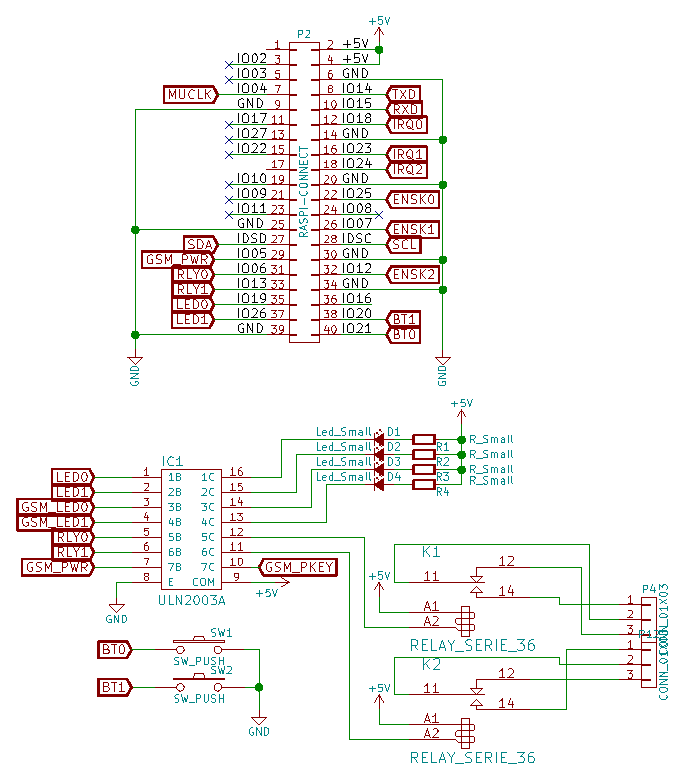
\includegraphics[width=0.725\textwidth]{images/superv-sch/supervisor--sch--gpio.eps}
    \caption[\Master: Schema GPIO]{GPIO \Master}
    \label{fig:sch:master:gpio}
\end{figure}

Das  \Master   besitzt  verschiedene  Ein-  und   Ausg\"ange. Kernst\"uck  des
GPIO-Blocks  ist  ein Darlington  Transistor  Array  (\code{IC1} in  Abbildung
\ref{fig:sch:master:gpio}),  welches verschiedene  Steuersignale durchschalten
kann.

Die  Signale  \code{LED0}  und  \code{LED1} steuern  die  LEDs  \code{D1}  und
\code{D2}  und  werden  vom  \Raspi~  gesteuert  und  dienen  dem  allgemeinen
Debugging. Signal  \code{GSM\_LED0}  respektive  \code{GSM\_LED1}  stehen  dem
GSM-Modem zur Statusausgabe zur Verf\"ugung.

Die   beiden  Relais   werden  von   \code{RLY0}  und   \code{RLY1}  gesteuert
und  k\"onnen  vom  Endbenutzer   f\"ur  beliebige  Funtionalit\"at  verwendet
werden. Daf\"ur stehen  die beiden  Anschl\"usse \code{P4} und  \code{P16} zur
Verf\"ugung.

Das Signal \code{GSM\_PWR} kann auf \code{GND} durchschalten, um das GSM-Modem
via den Pin  \code{GSM\_PKEY} einzuschalten, analog zu einem  Taster, um einen
PC einzuschalten.

Die  beiden  Anschl\"usse  \code{BT0}  und \code{BT1}  sind  mit  dem  \Raspi~
verbunden und k\"onnen f\"ur Jumper, Taster oder Schalter verwendet werden. In
der  Prototypenkonfiguration  ist   ein  Schalter  angeschlossen. Der  Stecker
\code{P2} ist die Hauptverbindung zum \Raspi via Flachbandkabel.

Als  IO-Verst\"arker  wird  ein   ULN2003A  von  Texas  Instruments  gew\"ahlt
\cite{datasheet:darlingtonic}. Der    IC    verf\"ugt    \"uber    integrierte
Freilaufdioden   zum    Schutz   vor    \"uberh\"ohter   Spannung    auf   der
Ausgangsseite. In unserem Fall dient  dies dazu, Spannungsspitzen, welche beim
Ausschalten der Relais auftreten k\"onnen,  abzufangen.  Da der \Raspi maximal
\SI{3.3}{\volt} am  Ausgang liefern  kann, muss  die Schaltschwelle  f\"ur ein
\code{true}-Signal bei diesem  IC bei \SI{3.3}{\volt} oder  tiefer liegen, was
der  ULN2003A erf\"ullt.   Die Relais  beziehen bis  zu \SI{72}{\milli\ampere}
\cite{datasheet:finder36relais}  Strom  bei   Betrieb  mit  \SI{5}{\volt}. Der
ULN2003A kann bis zu \SI{100}{\milli\ampere} pro Kanal liefern, was ausreichen
sollte, um die Relais zuverl\"assig schalten zu k\"onnen.

Die     Relais      sind     von      der     Serie     36      von     Finder
\cite{datasheet:finder36relais}. Sie  k\"onnen Lasten  bis zu  \SI{230}{\volt}
und  \SI{10}{\ampere}  schalten,  womit handels\"ubliche  Ger\"ate  f\"ur  das
Niederspannungsnetz angeschlossen werden k\"onnen. Dies gibt dem Kunden grosse
Flexibilit\"at bei der Wahl der  zu betreibenden Ger\"ate (Alarmlampe, Sirene,
\ldots).


% ---------------------------------------------------------------------------- %
\subsection{Kommunikation mit Sensoren}
\label{subsec:hw:master:sensorcomm}
% ---------------------------------------------------------------------------- %


\begin{figure}[h!t]
    \centering
    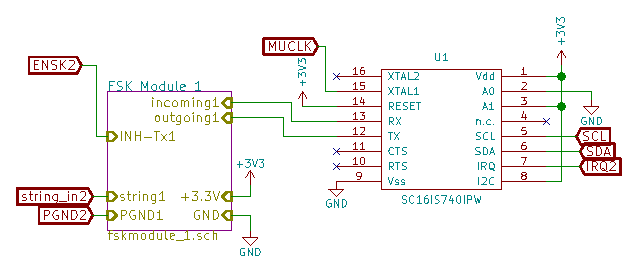
\includegraphics[width=0.75\textwidth]{images/superv-sch/supervisor--sch--comms.eps}
    \caption[\Master: Schema Kommunikation]{Kommunikation zu \Sensor auf \Master}
    \label{fig:sch:master:comms}
\end{figure}

Abbildung     \ref{fig:sch:master:comms}     zeigt    das     Schema     einer
der    drei     Schaltungen,    welche     zur    Kommunikation     mit    dem
Sensor    benutzt     werden. Zur    genauen    Beschreibung     des    Blocks
\code{fskmodule\_1.sch} siehe Abschnitt \ref{subsec:hw:sensor:transmitter} auf
Seite \pageref{subsec:hw:sensor:transmitter}.

Auf der rechten Seite in Abbildung \ref{fig:sch:master:comms} ist die Br\"ucke
\code{U1} abgebildet,  welche zwischen UART und  \ISC~konvertiert. Es wird das
Modell  SC16IS740 von  NXP Semiconructors  \cite{datasheet:uarti2c} verwendet.
Der \Sensor  sendet seine Daten  auf der DC-Leitung in  UART-Kodierung. Da der
\Raspi~nicht  gen\"ugend  UART-Eing\"ange  f\"ur alle  ben\"otigten  Leitungen
besitzt,  werden  die  Daten  im \ISC-Format  in  den  \Raspi~eingespeist. Die
Br\"ucke  \code{U1} ist  daf\"ur verantwortlich,  zwischen UART  (Anschl\"usse
\code{TX}  und \code{RX}  und  \ISC~(Anschl\"usse \code{SDA}  f\"ur Daten  und
\code{SDL} f\"ur Clock) zu konvertieren.

Den Clock erh\"alt die Br\"ucke vom Mikrocontroller des \Raspi~via die Leitung
\code{MUCLK}.

Wenn  von einem  \Sensor Daten  empfangen werden,  kann die  Br\"ucke mit  dem
Anschluss \code{IRQ2} einen Interrupt an den \Raspi~senden, welcher darauf die
Datenverarbeitung startet.

Die Pins  \code{A0} und  \code{A1} dienen der  Addressierung der  Br\"ucke und
sind f\"ur  jede Br\"ucke individuell angeschlossen. F\"ur  die vollst\"andige
Verdrahtung  siehe Seite
\pageref{fig:schema:master:full}
in Anhang
\ref{app:chap:schemas}

\fref{fig:sch:master:coupling} zeigt die  Anschl\"usse zur Einkopplung des
Signals auf die DC-Leitung. Es sind drei Stecker \code{P13} \code{P14} und
\code{P15}  vorhanden,  durch  welche  der  Strom  geleitet  wird. An  den
Steckern kann jeweils eine  Einkopplung angeschlossen werden. Dies erlaubt
Flexibilit\"at bei der  Implementierung der Einkopplung, da  das PCB nicht
auf eine spezifische Variante beschr\"ankt ist.

Die Ausg\"ange des Einkopplungsblocks gehen auf die Strommessung.
\begin{figure}[h!tb]
    \centering
    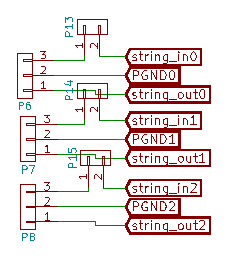
\includegraphics[width=0.25\textwidth]{images/superv-sch/supervisor--sch--coupling.eps}
    \caption[\Master: Schema Einkopplung]{Anschl\"usse zur Einkopplung}
    \label{fig:sch:master:coupling}
\end{figure}


% ---------------------------------------------------------------------------- %
\subsection{Strommessung}
\label{subsec:hw:master:current}
% ---------------------------------------------------------------------------- %


\begin{figure}[h!t]
    \centering
    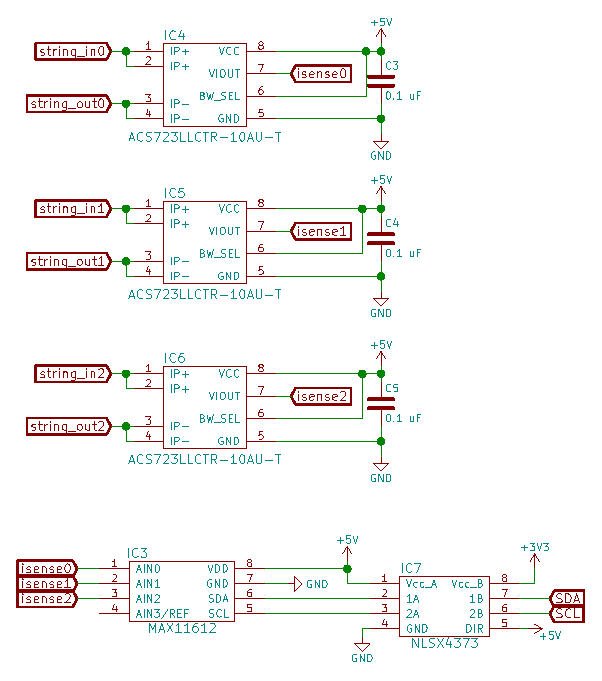
\includegraphics[angle=-90,width=0.60\textwidth]{images/superv-sch/supervisor--sch--current.eps}
    \caption[\Master: Schema Strommessung]{Strommessung}
    \label{fig:sch:master:current}
\end{figure}

Der  Strom jedes  Modulstrangs  wird separat  \"uberwacht;  die dazu  benutzte
Schaltung   ist   in   Abbildung   \ref{fig:sch:master:current}   dargestellt.
\code{IC4},  \code{IC5}  und  \code{IC6}  sind  die  Strommessungssensoren. Es
werden  Hall-Sensoren   der  Modellreihe   ACS725  von   Allegro  Microsystems
benutzt. Diese k\"onnen bis zu  \SI{10}{\ampere} messen, sind durchschlagsfest
bis zu  \SI{1}{\kilo\volt} und  k\"onnen sowohl  mit \SI{3.3}{\volt}  wie auch
\SI{5}{\volt} betrieben werden \cite{datasheet:hallic}.

Sie  geben   auf  den  Leitungen  \code{isense0},   \code{isense1}  respektive
\code{isense2}  eine   Spannung  aus,   welche  propotional  zum   den  Sensor
durchfliessenden Strom ist. Der vom Modulstrang  kommende Strom geht in in die
Eing\"ange \code{string\_in\{0,1,2\}} der Sensoren und verl\"asst diese wieder
durch die Ausg\"ange \code{string\_out\{0,1,2\}}, von wo der weitergeht in den
Generatoranschlusskasten.

\code{IC3}   ist    der   A/D-Konverter,   welcher   die    analogen   Signale
\code{isense0} bis \code{isense2} in  digitale Signale mit \SI{5}{\volt}-Pegel
wandelt. Es   kommt   ein   MAX11612   von  Maxim   Integrated   zum   Einsatz
\cite{datasheet:adc}. Dieser besitzt ein \ISC-Interface, drei Kan\"ale und ist
mit  dem  Ausgangspegel  der  Hall-Sensoren  kompatibel.   Allerdings  liefert
er  ein  Ausgangssignal  mit  einem \SI{5}{\volt}-Pegel,  was  nicht  mit  dem
\Raspi  kompatibel  ist, dessen  Eing\"ange  mit  einem Pegel  \SI{3.3}{\volt}
laufen. Deshalb wird zwischen \code{IC3} und  dem \Raspi noch ein Pegelwandler
der   Serie   NLSX4373  von   ON   Semiconductors   geschaltet,  welcher   das
\SI{5}{\volt}-Signal des ADC auf  \SI{3.3}{\volt} konvertiert. Er ist speziell
f\"ur  \ISC-Anwendungen entwickelt  worden  und eignet  sich  somit gut  f\"ur
unsere Zwecke.

Der Hersteller sieht zur  Stabilisierung der Stromversorgung einen Kondensator
der  Gr\"osse \SI{100}{\nano\farad},  sichtbar  im Diagramm  auf  Seite 1  des
Datenblattes \cite{datasheet:hallic}, vor.

% ---------------------------------------------------------------------------- %
\clearpage
\subsection{GSM-Modem}
\label{subsec:hw:master:gsm}
% ---------------------------------------------------------------------------- %

\begin{figure}[h!t]
    \centering
    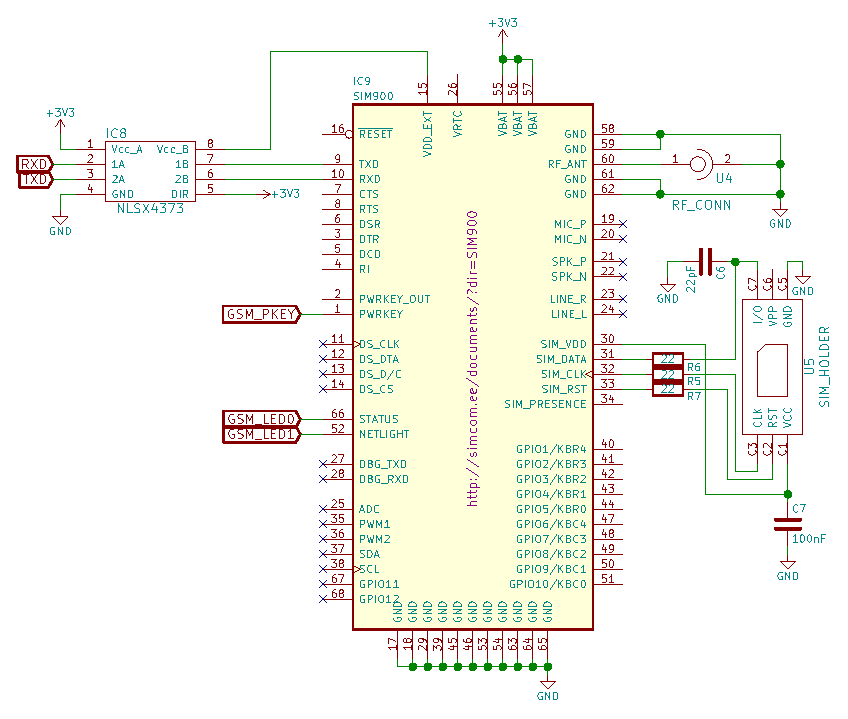
\includegraphics[width=0.85\textwidth]{images/superv-sch/supervisor--sch--gsm.eps}
    \caption[\Master: Schema GSM-Modem]{GSM-Modem Schaltung}
    \label{fig:sch:master:gsm}
\end{figure}

Das GSM-Modem  ist ein  integrierter Baustein,  der alle  n\"otigen Funktionen
bereitstellt; ein Baustein der SIM900-Serie von Simcom \cite{datasheet:modem}.
Er ist  zusammen mit seiner Beschaltung  in Abbildung \ref{fig:sch:master:gsm}
dargestellt. Wie auch  bei der  Strommessung wird  auch hier  ein Pegelwandler
verwendet, um  das Signal von der  UART-Linie mit \SI{3.3}{\volt} auf  den vom
GSM-Chip ben\"otigten  Pegel von \SI{2.8}{\volt} (Pin  \code{VDD\_EXT} auf dem
Chip, verbunden mit \code{Vcc\_B} auf dem Pegelwandler) zu wandeln.

Der  Pin  \code{GSM\_PKEY} dient  zum  Einschalten  des GSM-Modems,  gesteuert
vom  \Raspi  via  GPIO  (siehe  Abschnitt  \ref{subsec:hw:master:gpio},  Seite
\pageref{subsec:hw:master:gpio}).

Via die beiden Pins \code{STATUS}  und \code{NETLIGHT} werden zwei Status-LEDs
angesteuert (siehe  ebenfalls Abschnitt  \ref{subsec:hw:master:gpio}). Auf der
rechten Seite des  Schaltungsblocks ist die Antenne und der  Adapter f\"ur die
SIM-Karte zu sehen.

Gem\"ass  Referenzdesign  auf  Seite 9  des  Modem-Guides  \cite{ref:sim900:1}
betr\"agt der Wert aller Simkarten-Widerst\"ande \SI{22}{\ohm}.
